\documentclass[conference,letterpaper]{IEEEtran}
\usepackage[T1]{fontenc}
\usepackage[utf8]{inputenc}
\usepackage{amsmath,graphicx,booktabs,array,url,listings}
\graphicspath{{../resultados/final/}{../resultados/avance1/vibraciones/}{../resultados/avance2/diseno/}{../datos/}{../matlab/}}
\renewcommand{\abstractname}{Resumen}
\renewcommand{\refname}{Referencias}
\lstset{basicstyle=\ttfamily\footnotesize,breaklines=true,columns=fullflexible,keepspaces=true}
\newcommand{\fig}[2]{\begin{center}\includegraphics[width=\columnwidth]{#1}\\{\small #2}\end{center}}
\title{Vehículo autoguiado para mantenimiento predictivo con acople difuso y diagnóstico de rodamientos}
\author{\IEEEauthorblockN{Integrantes \underline{\hspace{5cm}}}
\IEEEauthorblockA{Ingeniería Mecatrónica, Universidad ECOTEC\\MEC451 Autómatas y Expertos · U3S7}}
\begin{document}
\maketitle
\begin{abstract}
Se implementó una red MLP para diagnosticar vibraciones en un vehículo de inspección de cinco estaciones. La entrada comprende nueve descriptores de ventanas CWRU de 2048 muestras a 12 kHz. La variante con 32 y 16 unidades ocultas logró 98,18\,\% en validación y 55 de 55 aciertos en prueba. En tres rondas de replay ROS~2, el primer destino cambió de E3 a E2 y luego a E5 tras el diagnóstico de falla de cada máquina. La misión física simulada en Gazebo completó las tres rondas y 15 acoples, con el mismo cambio de primer destino.
\end{abstract}
\begin{IEEEkeywords}
AGV, acople difuso, CWRU, mantenimiento predictivo, MLP, ROS~2.
\end{IEEEkeywords}
\section{Introducción}
El deterioro de rodamientos rotativos puede manifestarse en forma de cambios en la aceleración medida por el personal de mantenimiento. Una rutina semanal puede retrasar la observación de fallas. El vehículo autoguiado (AGV) busca automatizar el ciclo de inspección: decide a qué máquina acudir, estima su posición de acople, adquiere una ventana de vibración y usa el diagnóstico para actualizar prioridades.

La entrega integra los datos de planta, los módulos de decisión y el controlador difuso del repositorio previo. El objetivo de diagnóstico es identificar cuatro clases de vibración y alcanzar una exactitud mínima de 92\,\% sobre prueba temporal. El objetivo de integración es verificar que una falla detectada modifique el orden de la siguiente ronda.
\newpage
\subsection{Planta y alcance}
Las cinco placas de acople se distribuyen sobre el eje lateral de una planta de 5 × 4 m. El problema combina una decisión discreta (la próxima estación), una tarea continua (posición y orientación del vehículo) y una clasificación supervisada (tipo de vibración). El punto de medición queda a 10 cm de la placa según los sensores emulados. La máquina visitada se asocia a la ventana mediante el identificador de visita.

\fig{mapa_industrial.png}{Fig. 1. Mapa de la planta utilizado como antecedente de la misión.}
La tabla de distancias proviene de MATLAB. El lanzamiento U3S7 usa un seguidor odométrico para el pasillo conocido. El historial del proyecto registra dificultades de aproximación con Nav2/DWB. El trabajo actual corresponde a simulación, con el despliegue real en ESP32 previsto para la Unidad 4.
\clearpage

\section{Fase 1. Arquitectura y marco teórico}
\subsection{Vibración y fallas de rodamiento}
Una discontinuidad localizada excita la estructura cuando pasa el siguiente elemento rodante. El acelerómetro mide impactos amortiguados superpuestos a la componente de giro, al ruido y a otros modos mecánicos. La cadencia y la modulación varían con la ubicación del daño. Los descriptores temporales condensan escala e impulsividad y las bandas de energía complementan la información sobre frecuencia \cite{randall,smith}.

La curtosis de Pearson es el cuarto momento central normalizado por el cuadrado de la varianza. Para una distribución normal ideal vale tres. El exponente cuatro da mayor peso a valores extremos. El factor de cresta divide el máximo valor absoluto por el RMS. Ambos pueden aumentar si impactos breves amplifican el pico y la cola de la distribución. También pueden responder a una perturbación ajena al daño.

En un desbalance ideal domina la componente de giro 1×. Una sinusoide tiene curtosis 1,5 y factor de cresta $\sqrt{2}$ aun si aumenta su amplitud. Por eso estos dos cocientes pueden ser poco sensibles al crecimiento del desbalance. La energía en 1× es una opción para la extensión a Unidad 4.

\subsection{MLP y CNN unidimensional}
Una MLP aplica transformaciones densas con activaciones no lineales a entradas de longitud fija. RMS, pico y desviación recogen escala. Asimetría, curtosis y cresta recogen forma. Las energías por banda separan distribución espectral. Dada esta extracción previa, la red necesita unos cientos de coeficientes.

Una CNN 1D sobre la señal cruda sería pertinente si las formas transitorias o la periodicidad temporal aportaran información perdida al resumir cada ventana. El entrenamiento debería incluir más registros independientes y cargas y validar el presupuesto de cómputo \cite{lecun}.

\subsection{Comprobar arquitectura}
\begin{lstlisting}
python scripts/final/auditar_final.py
\end{lstlisting}
\newpage
\subsection{Geometría y control del acople}
A partir de las dos distancias filtradas a la placa se calculan:
\begin{align}
e_d &= (d_{fi}+d_{fd})/2-0{,}10,\\
e_\theta &= \arctan((d_{fi}-d_{fd})/0{,}20).
\end{align}
Un error angular positivo requiere velocidad angular negativa. Los rangos de una placa plana permiten estimar distancia y ángulo. Un vehículo paralelo desplazado lateralmente puede obtener los mismos rangos, de modo que el supervisor utiliza odometría para constatar el centrado. La secuencia difusa confirma $|e_d|\leq 0{,}01$ m y $|e_\theta|\leq5^\circ$ durante un segundo. La variante calibrada del controlador conserva las reglas Mamdani y los operadores mín--máx con defuzzificación por centroide \cite{mamdani}.

\fig{funciones_membresia.png}{Fig. 2. Funciones de membresía del controlador difuso base.}
\subsection{Orden de inspección}
El orden usa la primera regla aplicable. La falla tiene prioridad 1. Una estación de criticidad alta y más de cinco días sin inspección tiene prioridad 2. Baja criticidad en estado normal recibe prioridad 4. El caso general tiene prioridad 3. El menor coste desde la estación actual desempata y la etiqueta de estación hace determinista un empate restante.
\clearpage

\section{Metodología de datos}
Se empleó la aceleración del extremo de accionamiento (canal DE) a 0 hp \cite{cwru}. Las fallas tienen 0,007 pulgadas de diámetro. El archivo 97 es normal, 105 representa pista interna, 130 pista externa centrada a las 6:00 y 118 bola. La tabla de fuentes guarda URL, frecuencia usada, tamaño del registro y SHA-256. El normal se procesa a partir de 48 kHz y los tres registros de falla están a 12 kHz.

\subsection{División temporal}
Cada registro se corta en tres tramos contiguos del 70, 15 y 15\,\%. En el caso normal, el remuestreo con filtro antialias se aplica separadamente a cada tramo, para que el filtro de borde no mezcle las particiones. En cada tramo se toman ventanas de 2048 muestras con salto de 1024. Su duración a 12 kHz es 170,67 ms. El solapamiento del 50\,\% se limita a un mismo conjunto.

\begin{center}
\begin{tabular}{@{}lrrr@{}}
\toprule Clase & Entren. & Valid. & Prueba\\
\midrule Normal & 40 & 7 & 7\\
Pista interna & 81 & 16 & 16\\
Pista externa & 82 & 16 & 16\\
Bola & 82 & 16 & 16\\
\midrule Total & 285 & 55 & 55\\
\bottomrule
\end{tabular}\\
{\small Tabla I. Conteo por clase y conjunto.}
\end{center}
Las ventanas y las particiones se identifican por archivo, límites en muestras originales y desplazamiento dentro del tramo a 12 kHz. El menor número de ventanas normales se debe a la menor duración efectiva del registro tras remuestrear.
\newpage
\subsection{Vector de entrada}
Sea $x[n]$ la señal, $m_k$ su momento central de orden $k$ con divisor $N$ y $p=\max|x[n]|$. Se computan RMS, pico, curtosis $m_4/m_2^2$, asimetría $m_3/m_2^{3/2}$, desviación muestral con divisor $N-1$ y cresta $p/\mathrm{RMS}$. La FFT unilateral se escala por $N$ antes de elevar al cuadrado y se duplica la potencia de los bins interiores. Se conserva DC y Nyquist una vez. La resolución es 5,859 Hz. Las bandas $[0,1)$, $[1,3)$ y $[3,6]$ kHz suman la potencia media de la ventana según Parseval.

\fig{comparacion_final_fft_cwru_12k.png}{Fig. 3. Antecedente espectral de las cuatro clases a 12 kHz.}
\subsection{Escalamiento}
El escalador ajusta media y escala de cada descriptor con 285 ventanas de entrenamiento. Los parámetros se congelan al transformar validación, prueba y las ventanas que consume ROS~2. Se exportan junto a los pesos para conservar el orden exacto de las nueve entradas.
\clearpage

\section{Fase 2. Entrenamiento y validación}
Se comparan una capa densa de 32 neuronas y dos capas densas de 32 y 16. Ambas redes usan ReLU, un Dropout de 0,20 tras la primera capa y cuatro salidas Softmax. La red elegida tiene $9\cdot32+32+32\cdot16+16+16\cdot4+4=916$ parámetros, equivalentes a 3664 bytes de pesos y sesgos en 32 bits. También se debe presupuestar la memoria de la FFT y del búfer al migrar al ESP32.

\subsection{Protocolo de selección}
Los modelos usan TensorFlow/Keras \cite{tensorflow}, Adam \cite{adam} con tasa $10^{-3}$, entropía cruzada categórica, lotes de 32 y semilla 451. Se permitió hasta 100 épocas. La parada temprana vigila pérdida de validación desde la época 50 con paciencia de 12 y restauración de los mejores pesos supervisados. Ambas variantes alcanzaron las 100 épocas.

\begin{center}
\small
\begin{tabular}{@{}lrrr@{}}
\toprule Ocultas & Parámetros & Exactitud val. & Pérdida val.\\
\midrule 32 & 452 & 89,09\,\% & 0,20106\\
32--16 & 916 & 98,18\,\% & 0,09864\\
\bottomrule
\end{tabular}\\
Tabla II. Comparación sobre el conjunto de validación.
\end{center}
Un segundo entrenamiento en un entorno aislado reprodujo exactamente el resumen de métricas. El criterio primario de selección es la menor pérdida de validación. La mejora de 9,09 puntos porcentuales y la reducción aproximada de 51\,\% de pérdida justifican la segunda capa en este conjunto. El número de parámetros permite considerar un despliegue en el borde.
\newpage
\fig{curvas.png}{Fig. 4. Pérdida y exactitud a lo largo de las épocas.}
\subsection{Diagnóstico del ajuste}
Ambas curvas de pérdida descienden a medida que la red aprende los descriptores. La exactitud de validación de la segunda variante se aproxima al techo al final. Hay fluctuaciones en entrenamiento coherentes con el muestreo de lotes y el Dropout. La validación no muestra una divergencia sostenida de pérdida en el horizonte analizado. La segunda variante muestra buen ajuste en los tramos observados. Variaciones de carga, severidad, sensores y máquinas requieren una prueba adicional antes de estandarizar conclusiones operativas.

El Dropout está activo durante entrenamiento e inactivo en validación e inferencia. La pérdida se mide sobre la probabilidad de la clase real y puede variar aun cuando la exactitud permanezca igual. La exactitud describe decisiones discretas y la pérdida aporta señal adicional durante la selección.

\subsection{Reproducir entrenamiento}
\begin{lstlisting}
python -m pip install -r scripts/final/requirements.txt
python scripts/final/entrenar.py
python scripts/final/verificar.py --keras
\end{lstlisting}
\clearpage

\section{Fase 3. Evaluación del diagnóstico}
El conjunto de prueba se empleó después de seleccionar arquitectura. La exactitud fue 55/55, equivalente al 100\,\%, y supera la meta de 92\,\% dentro de esta partición. La matriz de confusión de 4 × 4 no presentó cruces. Precisión y sensibilidad fueron 1,00 para las cuatro clases. Los 7 ejemplos normales y los 16 de cada clase de falla tienen soporte desigual.

\fig{confusion.png}{Fig. 5. Matriz de confusión, con clase real por fila.}
\begin{center}
\begin{tabular}{@{}lrrr@{}}
\toprule Clase & Precisión & Recall & Soporte\\
\midrule Normal & 1,00 & 1,00 & 7\\
Pista interna & 1,00 & 1,00 & 16\\
Pista externa & 1,00 & 1,00 & 16\\
Bola & 1,00 & 1,00 & 16\\
\bottomrule
\end{tabular}\\
{\small Tabla III. Métricas en prueba.}
\end{center}
Precisión es VP/(VP+FP) y recall es VP/(VP+FN). El reporte conserva ambos indicadores incluso para la clase con menos observaciones.
\newpage
\subsection{Consistencia de inferencia}
El archivo Keras conserva la red entrenada. ROS~2 carga las matrices de pesos y los parámetros del escalador desde NPZ y ejecuta las capas densas, ReLU y Softmax con NumPy. La comparación de las 220 probabilidades de las 55 ventanas con Keras arrojó una diferencia absoluta máxima de $1{,}19\times10^{-7}$. Las clases predichas coincidieron en todos los casos.

\subsection{Contraste de características}
Se seleccionaron cinco ventanas del conjunto de prueba con representación de las cuatro clases. Se contrastaron los 45 valores de salida con una referencia NumPy/SciPy que implementa la curtosis de Pearson y la desviación con $N-1$. El máximo error relativo fue $1{,}22\times10^{-13}$\,\%. El script MATLAB lee las mismas cinco ventanas, usa momentos poblacionales equivalentes a \texttt{kurtosis(x,1)} y \texttt{skewness(x,1)}, calcula \texttt{std(x,0)} y exporta los 45 errores relativos \cite{matlab}. La verificación directa en MATLAB queda pendiente.


\subsection{Reproducir las cinco ventanas}
\begin{lstlisting}
python scripts/final/verificar.py
matlab -batch "addpath('matlab/final'); verificar_caracteristicas"
python scripts/final/auditar_final.py --matlab resultados/final/paridad_matlab.csv
\end{lstlisting}
\subsection{Interpretación}
En la prueba registrada no hubo clases confundidas. Como hipótesis para una futura prueba, bola y pista interna podrían solaparse en amplitud e impulsividad si cambian carga, sensor o montaje. Validar esa hipótesis requiere registros independientes representativos de ambos defectos. La presente exactitud caracteriza una combinación fija de banco, carga y diámetro.
\clearpage

\section{Fase 3. Integración y simulación}
El plan parte de Base en la primera ronda y de la última estación visitada en las rondas siguientes. Tras cada visita se actualiza el estado de prioridad con el diagnóstico y se recalcula el plan para pendientes. La regla de falla eleva una estación a prioridad 1. La matriz exportada desempata sin invocar MATLAB en línea.


\subsection{Compilar y lanzar en Humble}
\begin{lstlisting}
source /opt/ros/humble/setup.bash
export ROS_DOMAIN_ID=45 ROS_LOCALHOST_ONLY=1
colcon build --base-paths ros2_ws/src
source install/setup.bash
ros2 launch agv_avance3 avance3.launch.py \
  gui:=true registro:=rondas_video.jsonl
python scripts/final/validar_gazebo.py rondas_video.jsonl
\end{lstlisting}
\subsection{Secuencia de la misión}
La navegación final usa el pasillo conocido y la odometría para entrar centrada a cada estación. El emulador proyecta el LiDAR sobre dos bandas separadas 0,20 m. El inspector sincroniza los rangos por escaneo, filtra con $\alpha=0{,}3$ y verifica vigencia. El supervisor corrige sin avanzar si el rumbo excede $5^\circ$. El Mamdani actúa con rangos vigentes y la adquisición espera la confirmación geométrica sostenida. Tras un intento fallido puede volver al pasillo y reintentar. La adquisición se solicita al confirmar el acople.

\begin{center}
\small
\begin{tabular}{@{}p{2.2cm}p{5.4cm}@{}}
\toprule Componente & Flujo principal\\
\midrule Supervisor & Odometría y rangos a evento de acople.\\
Acelerómetro & Evento a ventana del banco de prueba.\\
Diagnosticador & Ventana a clase y confianza en ROS~2.\\
Priorizador & Clase a estado y nuevo orden de visita.\\
\bottomrule
\end{tabular}\\
Tabla IV. Intercambio de datos entre módulos.
\end{center}
El identificador de visita vincula evento, ventana y diagnóstico. El mensaje en \texttt{/diagnostico} contiene estación, ronda, ID, índice de ventana, clase y confianza. Se consume la respuesta de la visita activa y se registra su efecto en el plan.
\newpage
\subsection{Tres rondas en ROS 2}
Se ejecutó el replay con dos nodos que se comunican por los tópicos de ROS~2 Humble \cite{ros}. El verificador inyectó el evento de acople, comprobó identificadores e índices y siguió el nuevo plan. En la primera ronda, E2 presentó pista interna. En la segunda volvió a normal y se detectó bola en E5. En la tercera, E5 presentó pista externa. Para una falla nueva, la primera observación ocurre al visitar la estación. El primer destino cambia por el diagnóstico previo, como se observa en la tabla.

\begin{center}
\begin{tabular}{@{}cll@{}}
\toprule Ronda & Orden inicial & Falla observada\\
\midrule 1 & E3, E4, E1, E2, E5 & E2 interna\\
2 & E2, E3, E4, E1, E5 & E5 bola\\
3 & E5, E4, E3, E1, E2 & E5 externa\\
\bottomrule
\end{tabular}\\
{\small Tabla V. Orden confirmado mediante replay ROS~2.}
\end{center}
\fig{reordenamiento_ros.png}{Fig. 6. Primer destino por ronda. En naranja, la prioridad 1 derivada del diagnóstico anterior.}
Se verificaron quince diagnósticos vinculados a ventanas de prueba. El archivo JSON conserva clase y confianza por visita. El replay empleó eventos de acople inyectados. Luego se ejecutó el lazo completo en Gazebo Classic 11.10.2, sin interfaz gráfica. Los nodos usaron las mismas ventanas y reglas de prioridad.
\clearpage

\section{Discusión}
\subsection{Validez del conjunto de prueba}
La división temporal cumple la restricción de desunión de muestras. Ventanas de un mismo tramo pueden solaparse y todos los tramos proceden de los mismos cuatro registros. Un cambio de carga, ubicación, montaje o trayectoria de transmisión puede desplazar las distribuciones. Las siete ventanas normales corresponden a un registro de una sola condición. Los resultados se deben corroborar con nuevos archivos y particiones por máquina o condición \cite{smith}.

Las características espectrales añadidas reflejan el dominio de muestreo y los registros de laboratorio. Si cambia el muestreo, es necesario redefinir las bandas. La futura verificación en ESP32 debe registrar latencia de adquisición, extracción, normalización e inferencia. El tamaño reducido de la MLP es un indicador inicial de viabilidad y la FFT puede dominar el presupuesto de trabajo.

\subsection{Validez del lazo de inspección}
El replay verifica transporte, contrato de datos y reacción causal del orden de visita. El simulador añade cadencia de odometría, rayos LiDAR, contacto, ruido, reintentos y condiciones de parada. El umbral de acople se analizó en ensayos separados de la misión nominal. Los resultados numéricos históricos se conservan como antecedentes. En Gazebo se completaron las 15 visitas en el mismo orden del replay. La repetición en WSL con interfaz duró 134,994 s de pared. El máximo error final fue 7,46 mm y 4,38 grados. Se registraron cero reintentos sobre 15 visitas y 9,63 s simulados en promedio por acople. La desviación lateral final máxima fue 8,17 mm. El criterio longitudinal y angular se confirmó en las 15 visitas. La corrida corresponde al escenario nominal de tres rondas.

Para el Waffle se ajustó el parámetro de rampa de rueda del complemento de Gazebo a cero después de observar un retraso entre consigna de giro y odometría. La simulación conservó el control diferencial y los límites de velocidad del supervisor. El seguimiento por pasillo es específico del tablero conocido. Una planta dinámica requeriría detección de obstáculos y un planificador de movimiento capaz de replantear trayectorias con las nuevas restricciones.
\subsection{Criterio de acople y reproducción}
Cinco intentos por caso, con reinicio de pose en E1, ruido de rango habilitado y un intento por repetición. La base se colocó en $x=0{,}76$ m, a unos 0,51 m de la placa desde la línea de sensores. La primera prueba con espera de rangos y sin realineamiento obtuvo 11/15. A $15^\circ$, la geometría puede situar una proyección lateral fuera del borde de la placa. El ajuste limita el realineamiento por odometría a la zona de preacople, con velocidad lineal nula. El lote definitivo alcanzó 15/15 sin reintentos.
\begin{center}\small
\begin{tabular}{@{}lrrr@{}}
\toprule Escenario & Éxitos & $|e_d|$ mm & $|e_\theta|$ deg\\
\midrule
Frontal & 5/5 & 9,50 & 3,85\\
Giro de $15^\circ$ & 5/5 & 5,99 & 4,20\\
Residual $3$ cm / $10^\circ$ & 5/5 & 7,32 & 3,12\\
\bottomrule
\end{tabular}\\
Tabla VI. Errores máximos por escenario.
\end{center}
\begin{lstlisting}
ros2 launch agv_avance3 avance3.launch.py \
  gui:=false ensayos:=true registro:=acople.jsonl
python scripts/final/validar_ensayos.py acople.jsonl
\end{lstlisting}
\subsection{Trazabilidad de evidencia}
\begin{center}
\small
\begin{tabular}{@{}p{3cm}p{4.5cm}@{}}
\toprule Evidencia & Alcance\\
\midrule Clasificación & 55 ventanas temporales.\\
Keras--NumPy & 220 probabilidades contrastadas.\\
NumPy--SciPy & 45 características contrastadas.\\
MATLAB--Python & Script y tablas de entrada preparados.\\
Replay ROS~2 & 15 diagnósticos y tres planes iniciales.\\
Gazebo & 15 acoples y diagnósticos en tres rondas.\\
\bottomrule
\end{tabular}\\
Tabla VII. Cobertura de las comprobaciones.
\end{center}

\begin{center}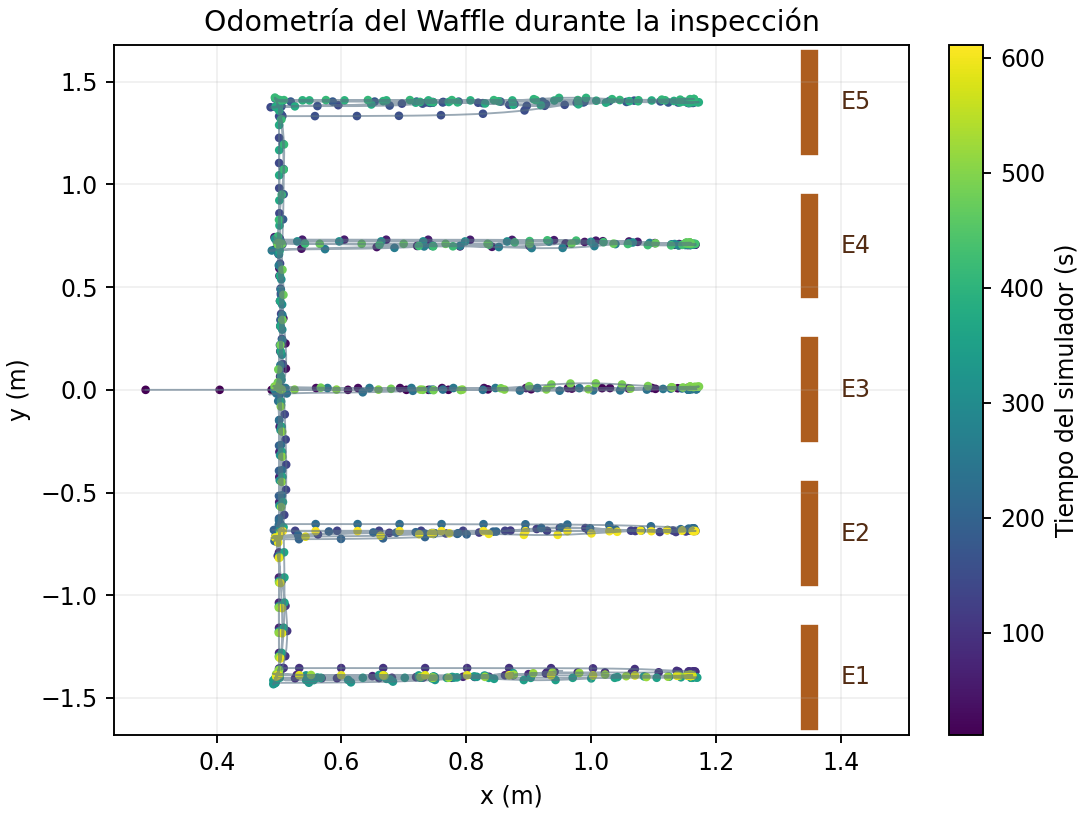
\includegraphics[width=.78\columnwidth]{gazebo_trayectoria.png}\\{\small Fig. 7. Trayectoria de la primera misión completa en Gazebo.}\end{center}
\subsection{Próxima extensión en ESP32}
Los datos de un MPU6050 sobre prototipos con desbalance provendrán de un dominio mecánico distinto. Se necesitará un banco propio, particiones por sesión y análisis de la componente de giro 1×. En el microcontrolador, la reducción de precisión de los pesos requiere calibración y medición directa del impacto sobre exactitud y memoria. Se propone medir latencia extremo a extremo con FFT y adquisición incluidas.

\subsection{Reproducción de los resultados}
El manifiesto con SHA-256 identifica el origen de los datos. El CSV conserva tramos y desplazamientos. El banco NPZ expone las mismas ventanas a ROS~2, a la verificación de probabilidades y al verificador de cinco ventanas. Para auditar el proceso se repiten el entrenamiento y el replay con las rutas de archivo descritas en el repositorio.
\clearpage

\section{Conclusiones}
La MLP con estructura 9--32--16--4 obtuvo menor pérdida de validación que la de una capa. Con 916 parámetros, logró 55 aciertos de 55 ventanas de prueba del conjunto CWRU a 0 hp. No se observaron confusiones en las cuatro clases. Los resultados proceden de tramos temporales disjuntos de los mismos registros y deben verificarse con nuevos motores y cargas.

El flujo ROS~2 procesó las quince visitas de replay. Tras confirmar pista interna en E2 y falla de bola en E5, el primer destino pasó de E3 a E2 y luego a E5. Esta prueba respalda la actualización de prioridades con la clase recibida por tópicos. Gazebo confirmó la misma evolución del orden inicial y registró las quince visitas. Se preparó el script para ejecutar el contraste directo en MATLAB.

El modelo exportado conserva escalas y orden de entrada. La comparación de las probabilidades con el modelo de entrenamiento muestra que se puede desplegar el clasificador fuera del entorno TensorFlow sin alterar las decisiones observadas. El siguiente paso del proyecto estudiará el muestreo propio, la medida 1× y la latencia integral en ESP32.

\subsection{Exportar video y compilar el informe}
\begin{lstlisting}
bash entrega_final/exportar_video.sh \
  gazebo_bruto.mkv Video_Final.mp4
(cd entrega_final && latexmk -pdf informe.tex)
\end{lstlisting}
La guía \texttt{COMPILACION\_Y\_VIDEO.md} contiene la instalación, los tópicos de inspección, el comando de captura X11 y la alternativa para Wayland o WSL. La edición final se limita a 180 s.
\newpage
\begin{thebibliography}{00}
\bibitem{randall} R. B. Randall y J. Antoni, “Rolling element bearing diagnostics---A tutorial,” \emph{Mechanical Systems and Signal Processing}, vol. 25, n.º 2, pp. 485--520, 2011. doi: 10.1016/j.ymssp.2010.07.017.
\bibitem{smith} W. A. Smith y R. B. Randall, “Rolling element bearing diagnostics using the Case Western Reserve University data: A benchmark study,” \emph{Mechanical Systems and Signal Processing}, vols. 64--65, pp. 100--131, 2015. doi: 10.1016/j.ymssp.2015.04.021.
\bibitem{lecun} Y. LeCun, Y. Bengio y G. Hinton, “Deep learning,” \emph{Nature}, vol. 521, pp. 436--444, 2015. doi: 10.1038/nature14539.
\bibitem{mamdani} E. H. Mamdani y S. Assilian, “An experiment in linguistic synthesis with a fuzzy logic controller,” \emph{International Journal of Man-Machine Studies}, vol. 7, n.º 1, pp. 1--13, 1975. doi: 10.1016/S0020-7373(75)80002-2.
\bibitem{cwru} Case Western Reserve University, “Bearing Data Center, Download a Data File.” \url{https://engineering.case.edu/bearingdatacenter/download-data-file}
\bibitem{tensorflow} M. Abadi \emph{et al.}, “TensorFlow: A system for large-scale machine learning,” en \emph{USENIX OSDI}, pp. 265--283, 2016.
\bibitem{adam} D. P. Kingma y J. Ba, “Adam: A method for stochastic optimization,” \emph{ICLR}, 2015. \url{https://arxiv.org/abs/1412.6980}
\bibitem{matlab} MathWorks, “kurtosis” y “std,” documentación de MATLAB. \url{https://www.mathworks.com/help/stats/kurtosis.html}
\bibitem{ros} Open Robotics, “ROS 2 Humble documentation.” \url{https://docs.ros.org/en/humble/}
\end{thebibliography}
\end{document}
